\RequirePackage[2020-02-02]{latexrelease} % workaround for broken
\documentclass[10pt,a4paper]{article}
% ========================== DO NOT MODIFY =================================== %
\usepackage[a4paper,left=2.0cm,top=2.0cm,right=2.0cm,bottom=2.0cm]{geometry}
\usepackage{amssymb,amsmath} % If amsmath is required
\usepackage[implicit=false]{hyperref}
\usepackage[utf8]{inputenc}
\usepackage[T1]{fontenc}
\usepackage{times}
\usepackage{graphicx}
\usepackage{titling}
\usepackage{authblk}
\usepackage{multicol}
\usepackage{float}
\usepackage{enumitem}
\usepackage{booktabs}
\usepackage{xcolor}
\usepackage{hyperref}
\hypersetup{
    colorlinks=true,
    linkcolor=blue,
    filecolor=blue,      
    urlcolor=blue,
}
    
\usepackage{fancyhdr}
\fancyhf{}
\setlength{\headheight}{3em}
\pagestyle{fancy}
\renewcommand{\headrulewidth}{0pt} % remove lines as well
\fancyhead[L]{\footnotesize{24\textsuperscript{th} International Conference on Biomedical Applications of Electrical Impedance Tomography (EIT 2024), Hangzhou, China}}
\fancypagestyle{firstpage}{%
  \lhead{\footnotesize{24\textsuperscript{th} International Conference on Biomedical Applications of Electrical Impedance Tomography (EIT 2024),  Hangzhou, China}}
}

\usepackage[small,compact]{titlesec}
% Fix titlesec for the 2.10.1 version in ubuntu 16.04
%  https://bugs.launchpad.net/ubuntu/+source/texlive-extra/+bug/1574052
\makeatletter
\@ifpackagelater{titlesec}{2016/03/21}{%
 % Package titlesec is on version 2.10.2 or higher, nothing to do %
}{%
 % Check if package titlesec is on version 2.10.1 %
 \@ifpackagelater{titlesec}{2016/03/15}{%
  % Package titlesec on version 2.10.1, patch accordingly %
  \usepackage{etoolbox}%
  \makeatletter
  \patchcmd{\ttlh@hang}{\parindent\z@}{\parindent\z@\leavevmode}{}{}%
  \patchcmd{\ttlh@hang}{\noindent}{}{}{}%
  \makeatother
 }{%
  % Package titlsecon is on version 2.10.0 or lower, nothing to do %
 }%
}
\makeatother
\titlespacing*{\section}{0pt}{5pt}{5pt}  % If you need different spacing

\usepackage[numbers,sort&compress]{natbib}
\usepackage[small,bf,tableposition=top,figureposition=bottom,skip=2pt]{caption}


% limit space between floats and text
\setlength{\textfloatsep}{10pt plus 1.0pt minus 2.0pt}
% shrink the list environments
\setlist{noitemsep}
\setlist{nolistsep}

% Shrink the bibliography
  \let\oldthebibliography=\thebibliography
  \let\endoldthebibliography=\endthebibliography
  \renewenvironment{thebibliography}[1]{%
    \begin{oldthebibliography}{#1}%
      \setlength{\parskip}{0ex}%
      \setlength{\itemsep}{0ex}%
  }%
  {%
    \end{oldthebibliography}%
  }

% Format of the front matter
\renewcommand{\Affilfont}{\small}
\setlength{\affilsep}{1ex}
\renewcommand\Authands{, }
\setlength{\droptitle}{-2cm}
% ============================================================================ %




%------------------------------- FRONT MATTER -------------------------------- %
\title{EIDORS Version 3.12%
\vspace{-0.5ex}} %remove vertical space
\author[1]{Andy Adler}
\author[1]{Bartłomiej Grychtol}
\affil[1]{Systems and Computer Engineering, Carleton University, Ottawa, Canada, \protect\href{mailto:adler@sce.carleton.ca}{\underline{adler@asce.carleton.ca}}}
\date{}
%----------------------------------------------------------------------------- %
%\protect\url


\begin{document}
\maketitle
\thispagestyle{firstpage}
\vspace{-1.5cm}
%\thispagestyle{empty}

\begin{multicols}{2}

\noindent {\bf Abstract:}
This paper announces the release of version 3.12 of the
EIDORS software suite. We review its new features, and 
discusses its growth and use.

\section{Introduction}
We proudly announce the release of EIDORS version 3.12,
for the 24th Int.\ Conf.\ on Biomedical Applications of EIT,
in July 2024.
The software is available at \href{www.eidors.org}{eidors.org}\, and licensed under the GNU GPLv2 or GPLv3. Archived versions are now available on Zenodo
\cite{eidors3p11,
      eidors3p10,
      eidors3p9p1,
      eidors3p9,
      eidors3p8}, and all versions available on 
\href{www.sourceforge.net}{sourceforge.net}
\cite{adler2005, adler2006, adler2008, adler2015, adler2017}


EIDORS provides free software algorithms for forward modelling
and inverse solutions
of Electrical Impedance and (to some extent) Diffusion-based Optical Tomography, in
medical, industrial and geophysical settings.
EIDORS also aims to share data and promote
collaboration.

\section{New Features}
Release 3.12 of EIDORS builds upon a strong foundation in reconstruction
algorithms, adding and improving a number of aspects.
\begin{itemize}
\item D-bar solver with Dirichlet-Neumann estimation
\item New data formats (Sciospec and HDF5)\cite{possner2023hdf5}
\item Improved solver preconditioning
\item Improved Octaves support
\item New faster hash (xxHash) for object caching
\item Improved Control of netgen refinement
\item 3D perfusion and $\dot{\rm V}$/Q analysis tools\cite{araos2023VQ}
\item Improved FFT-based filtering functions
\item Expanded data contributions (e.g.~fig.2)
\item Improved Instrument models
\item Expanded shape library with new species shapes

\item (As always) bug fixes 
\end{itemize}

\section{Growth}
EIDORS-related citations continue to grow. Current citation results are
shown in
 table~1.  %table~\ref{tbl:cite}.
%
The EIDORS code-base is growing
%(fig.~\ref{fig:loc})
(fig.~1)
 with significant effort being applied to
improving test coverage, refining performance and implementing new features.
 In 2012, a {\tt dev} (development) staging area was created for
contributions in progress.

\begin{table}[H]
  \footnotesize
\centering
%From: http://amath.colorado.edu/documentation/LaTeX/reference/tables/ex1.html
\caption{EIDORS Citations
 (May 2024, scholar.google.com).
}
\label{tbl:cite}
\begin{tabular}{r@{\hspace{1mm}}lcr}
  \toprule
  & Paper & Date & \hspace{-2mm}Citations \\
  %{@{\extracolsep{\fill}}@{}|c|ccc|r|}
  \midrule
  \cite{vauhkonen2001} & A MATLAB package for the EIDORS project \ldots\hspace{-5mm}  
    & 2001 & 336 \\
  \cite{polydorides2002phd} & Image reconstruction algorithms for \ldots
    & 2002 & 194 \\
  \cite{polydorides2002matlab} & A Matlab toolkit for three-dimensional \ldots
    & 2002 & 564 \\
  \cite{adler2005} & EIDORS: Towards a community-based \ldots
    & 2005 & 38 \\
  \cite{adler2006} & Uses and abuses of {EIDORS}: An extensible \ldots
    & 2006 & 956 \\
  \cite{adler2008} & Simple FEMs aren't as good as we thought \ldots
    & 2008 &  26 \\
  \cite{adler2017} & EIDORS version 3.9
    & 2017 & 34 \\
  \cite{adler2017} & EIDORS version 3.10
    & 2019 & 5 \\
  \bottomrule
\end{tabular}
\vspace{-1em}
\end{table}

\begin{figure}[H]
  \vspace{-2.5mm}
\centering
% trim=left botm right top
 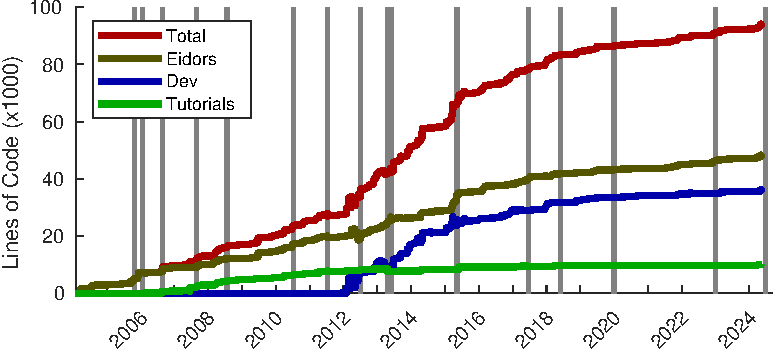
\includegraphics[width=.99\columnwidth]{fig_loc.pdf}
\caption{%
%graph and table combo chart, including line for test code.
  Lines of Code (LoC) in Matlab files in the EIDORS code-base vs.\ time; Total
   (red), EIDORS (i.e.\ release branch, brown), Tutorials (green), development code (blue).
   Releases are indicated by gray bars (The 3.12 release is
   at the right).
}
\label{fig:loc}
\end{figure}


\begin{figure}[H]
  \vspace{-2.5mm}
\centering
% trim=left botm right top
 \includegraphics[width=.99\columnwidth]{horse-3D.pdf}
\caption{%
%graph and table combo chart, including line for test code.
Transverse, saggital and oblique slices of 3D EIT images of a horse:
Rebreathing leads to increased respiratory rate and tidal volume.
}
\label{fig:horse}
\end{figure}

\section{Discussion}
The structure of EIDORS has been relatively stable due, in part, to some early design choices:
a modular framework and data structure,
cross-platform support, integration of meshing,
tutorials, and the contributed data repository.
These aspects, along with an open source code-base, have enabled EIDORS to
maintain research relevance.
Version 3.12 (hopefully) continues the tradition.






\footnotesize
% Instead of using thebibliography, you can also type the references
% using bibtex, and uncomment the following lines
%\bibliographystyle{compact}
%\bibliography{eit2018}
\begin{thebibliography}{}
\bibitem{eidors3p11}
   Adler A, ``EIDORS v3.11'',
   \href{http://dx.doi.org/10.5281/zenodo.7495740}{DOI:10.5281/zenodo.7495740},
    2019.
\bibitem{eidors3p10}
   Adler A, ``EIDORS v3.10'',
   \href{http://dx.doi.org/10.5281/zenodo.3247168}{DOI:10.5281/zenodo.3247168},
    2019.
\bibitem{eidors3p9p1}
   Adler A {\em et al}, ``EIDORS v3.9.1'',
   \href{http://dx.doi.org/10.5281/zenodo.1257670}{DOI:10.5281/zenodo.1257670},
    2018.
\bibitem{eidors3p9}
   Adler A {\em et al}, ``EIDORS v3.9'',
   \href{http://dx.doi.org/10.5281/zenodo.583266}{DOI:10.5281/zenodo.583266},
    2017.
\bibitem{eidors3p8}
   Adler A {\em et al}, ``EIDORS v3.8'',
   \href{http://dx.doi.org/10.5281/zenodo.17559}{DOI:10.5281/zenodo.17559},
    2015.

\bibitem{araos2023VQ}
   Araos J, \emph{et al}, 
``$\dot{\rm V}$/Q analysis with 3D EIT'',
p25, Conf EIT 2023.

\bibitem{possner2023hdf5}
   Possner L, \emph{et al}, 
``HDF5-based data format \ldots'',
p39, Conf EIT 2023.



\bibitem{vauhkonen2001}
   Vauhkonen \& M,  {\em  et al},
%  Vauhkonen \& M, Lionheart WRB {\em  et al},
   {\em  Physiol Meas}, 22:107--111, 2001.

\bibitem{polydorides2002phd}
   Polydorides N,
%{\em Image Reconstruction Algorithms for Soft-Field Tomography},
 {\em Ph.D. thesis}, U Manchester, UK, 2002.
\bibitem{polydorides2002matlab}
   Polydorides N, Lionheart WRB,
   {\em Meas Sci Tech}, 13:1871--1883, 2002.
\bibitem{adler2005}
Adler A, Lionheart WRB,
%"EIDORS: Towards a community-based extensible software base for EIT." 6th Conference on Biomedical Applications of Electrical Impedance Tomography, London, UK. 2005.
{\em Proc EIT2005}, London, UK, 2005.
%
\bibitem{adler2006}
Adler A, Lionheart WRB,
{\em Physiol Meas} 27:S25--S42, 2006.

\bibitem{adler2008}
Adler A, Borsic A {\em et al},
%Simple FEMs aren't as good as we \ldots
{\em Proc EIT2008}, Hannover, NH, USA, 2008.
\bibitem{adler2015}
Adler A {\em et al}, %Alistair Boyle, Michael G Crabb, Hervé Gagnon, Bartłomiej Grychtol, Nolwenn Lesparre, William R.B. Lionheart,
\href{https://zenodo.org/record/17752}{\em Proc EIT2015}, p.19, 
 Neuchâtel, Switzerland, 2015.

\bibitem{adler2017}
Adler A {\em et al}, % Andy Adler, Alistair Boyle, Fabian Braun, Michael G. Crabb, Bartłomiej Grychtol, William R. B. Lionheart, Henry F. J. Tregidgo, Rebecca Yerworth
\href{https://zenodo.org/record/557093}{\em Proc EIT2017}, p.63, 
Dartmouth, NH, USA,  2017.
\end{thebibliography}
\end{multicols}



\end{document}
